\chapter{Motion blur}
\label{ch:mb}
In the vast majority of real-world applications, neither the camera nor the scene remain stationary.
A static snapshot of the scene, therefore, fails to capture any motion taking place.
Consequently, rapid motion in the scene or of the camera cannot be accurately represented without increasing the frame rate.
This lack of representation results is temporal aliasing between frames, which is jarring and disorienting for the viewer.
This effect is particularly exacerbated in interactive applications as there is no control of the camera.
As such multiple approaches to reduce temporal aliasing, in application where computational resources and thus frame rates are limited, have been developed.

\section{Geometry substitution}
\label{ch:mb-gs}
An alternative approach to reduce temporal aliasing by increasing the frame rate involves modifying the underlying geometry to approximate a moving object.
The geometry and its texture are "smeared" across multiple time steps, while only one image is captured.
These methods work by approximating the equation \ref{eq:mb-cg-integral} to 

\begin{align}
    I_{xy} \approx \sum_{l'} \int_\Omega r_s(\omega)g_{l'}'(\omega)L_{l'}'(\omega) \: d\omega
    \label{eq:mb-geo-approx}
\end{align}

In equation \ref{eq:mb-geo-approx} the geometry $l$ is replaced by an alternative geometry $l'$ and all other functions are replaced by time-independent replacements.
As such this approach can referred to as a geometry post-processing effect, because it operates in object rather than in image space.

The first method implementing this approach was presented by Wloka et al. \cite{Wloka.1996} and demonstrates the basic method.
Their method begins by calculating the motion vector of an objects motion relative to the camera using the equation

$$
v_{obj} = (pos_{cam}(t_1) - pos_{cam}(t_0)) - (pos_{obj}(t_1) - pos_{obj}(t_0).
$$

This vector is then transformed to object space to operate on the object.
For the linear movement between the timesteps $t_0$ and $t_1$, $v_{obj}$ defines a front and back half of the object:

\begin{align}
    FrontPolygons &= \{ p |  Normal(p) \cdot v_{obj} \geq 0 \} \\
    BackPolygons  &= \{ p |  Normal(p) \cdot v_{obj} < 0 \}.
\end{align}

To ensure coherency and of the resulting motion volume, the object at timestep $t_1$ is used in the following steps.
The back half of polygons are moved by $-v_{obj}$ to the starting position of the motion and connected to the front half, as illustrated in figure \ref{fig:object-splitting}.
Alternatively, the transformation matrix, of the previous frame, is used for $FrontPolygons$ and the current transformation matrix for $BackPolygons$.

\begin{figure}
    \centering
    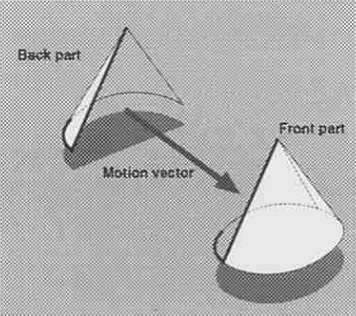
\includegraphics[width=0.4\textwidth]{images/object-splitting.png}
    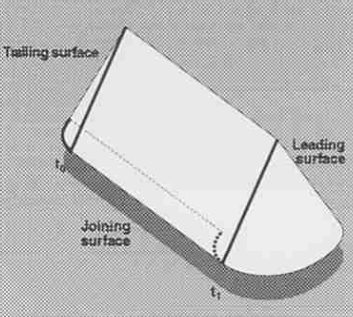
\includegraphics[width=0.4\textwidth]{images/object-splitting-assembly.png}
    \caption{Disassembly of object and construction of motion volume \cite{Wloka.1996}}
    \label{fig:object-splitting}
\end{figure}

Finally the transparency of the resulting motion volume is varied across its length to simulate a convincing motion blur.
A variety of functions are available to the artist to simulate different accelerations or shutters.
To represent non-linear motion the joining surface may be split at additional points to approximate curves \cite{Wloka.1996}.

Since this method can be executed by the vertex shader, its performance is very high.
However, the basic implementation of this approach comes with various limitation that preclude its use in modern applications.
The most significant constraints include the missing support for polygons with genus higher than zero (i.e., a torus) and rotation.
Additionally any real-time shadows calculated for the moving object must consider the transparency added to the motion volume by its motion.
Nevertheless, this simple method plays an important part in the approach discussed in section \ref{ch:mb-mf}.

\section{Accumulation buffers}
\label{ch:mb-acc}
The closest approximation of motion blur using traditional rendering pipelines can be achieved by the use of accumulation buffers.
This method is relatively easy to understand and implement.
A hardware buffer is used to average over $N$ rendering passes at different time steps.
The equation \ref{eq:mb-cg-integral} is approximated as

\begin{align}
    I_{xy} \approx \sum_{i=0}^{N-1} \frac{1}{N} \sum_{l} \int_\Omega f(\omega, t_i) g_l(\omega, t_i) L_l(\omega, t_i) \: d\omega.
\end{align}

Each individual frame is added with a factor of $\frac{1}{N}$, but these factors can be adjusted if a particular effect is desired.
With higher values of $N$ this method approaches the correct solution, but only displays a new image every $N$ rendering passes.
In many application this results in an unacceptable loss of performance \cite{Haeberli.1990}.

If higher update rates are desired and all frames are added with the same factor, filtering by repeated integration can be used \cite{Heckbert.1986}.
Initially $N$ frames are rendered normally and the resulting image is displayed.
To generated the next image, the first frame is rendered again and subtracted from the accumulation buffer.
Then frame $N+1$ is rendered and added to the accumulation buffer.
With this method a new image is displayed for every two frames rendered \cite{Haeberli.1990}.

\section{Motion fields}
\label{ch:mb-mf}
Motion fields provide another method to alleviate temporal aliasing, using the concept of vector fields to represent motion in the scene.
Similar to depth fields, motion fields supply additional information to image space algorithms by capturing the direction and magnitude of movement in the scene.

The basic idea behind motion fields is to record the motion vector in screen space at every pixel in the image for the duration of a frame.
This is accomplished in a vertex shader by transforming each vertex to window coordinates using the current and previous transformation matrix.
This results in two 2D-vectors $(x_s,y_s)$ and $(x_d,y_d)$ for the source and destination coordinates of a vertex.
The resulting movement vector of $(x_r,y_r) = (x_d - x_s,y_d - y_s)$ can be used directly or divided by $dt$ to get the screen space velocity.

The recorded motion field can then be used in several ways.
One straightforward application is to interpolate it across the geometry and pass that information to the pixel shader.
It would then 'smear' the image along the motion vectors, simulating a type of motion blur.
This can be mathematically represented as:

\begin{align}
    I_{xy} &= \frac{1}{N} \sum_{i=0}^{N-1}  S(x_s + x_r \frac{i}{N-1}, y_s + y_r \frac{i}{N-1}),
    \label{eq:mb-mf-approx}
\end{align}
where $S$ represents the rendered starting image.
Again the factors of $1/N$ may be adjusted to other filters (e.g. Gaussian or ramp) to simulate different types of motion.

This simple approach can be done in a single rendering pass.
However this simple approach does not provide no velocity information outside the silhouette of an object.
As a result, the blur is also confined to the object's silhouette, leading to an unnatural and distracting effect.

Green \cite{Green.2003} offers a solution to this issue, utilizing the geometric substitution introduced by Wloka \cite{Wloka.1996}, discussed in section \ref{ch:mb-gs}
Initially, a normal rendering pass is performed and stored as texture, without calculating screen space velocities.
Next a second rendering pass is done with the geometry stretched along its movement.
During this pass, no color information is rendered, only the screen space velocity is calculated and interpolated over the now stretched geometry.
The resulting velocity map is then used in calculating equation \ref{eq:mb-mf-approx} in a final pixel shader pass.
The second rendering pass of the motion field may be done at a smaller resolution to help with performance and blurring of edges \cite{Sousa.2008}.

It's important to note that, like the previous methods, the use of motion fields involves trade-offs. 
While it can produce visually pleasing results for a variety of motion effects, it also lacks proper support for rotation.
Here it relies on the short visibility of each frame to hide any generated artefacts.
Nevertheless, the flexibility and power of the motion field approach make it an important tool in the arsenal for reducing temporal aliasing.